\input{settings}
\setlength{\emergencystretch}{2em}
\titleformat{\section}
  {\small\bfseries\raggedright}
  {}{0em}
  {}
  [{\color{WHU_Blue}\titlerule}]
\titlespacing*{\section}{0cm}{0.85em}{0.60em}
\titlespacing*{\subsection}{0cm}{0.50em}{0.30em}
\setlist[itemize]{topsep=0.20em, itemsep=0.20em, parsep=0em, partopsep=0em, leftmargin=1.25em}
\setlist[enumerate]{topsep=0.20em, itemsep=0.20em, parsep=0em, partopsep=0em, leftmargin=1.35em}
\renewcommand{\arraystretch}{0.98}
\renewcommand{\CJKglue}{\hskip 0.018em}

% 个人信息
%  cd C:\Users\31087\Documents\Obsidian_Vault\Resume\template
%  xelatex main.tex
\newcommand{\school}{江南大学 · 控制科学与工程}

\newcommand{\resumeDecor}{
    \begin{tikzpicture}[remember picture, overlay]
        \node[anchor=north, inner sep=0pt](header) at (current page.north){
            
\includegraphics[width=\paperwidth]{images/header.png}
        };
        \node[anchor=west](school_logo) at (header.west){
            \hspace{0.5cm}
            
\includegraphics[width=0.15\textwidth]{images/whu_logo_1.png}
        };
        \node[anchor=east](school_name) at(header.east){
            \textcolor{white}{\textbf{\school}}
            \hspace{0.5cm}
        };
    \end{tikzpicture}

    \begin{tikzpicture}[remember picture, overlay]
        \node[opacity=0.05] at(current page.center){
            
\includegraphics[width=0.68\paperwidth, keepaspectratio]{images/whu_logo_big.png}
        };
    \end{tikzpicture}
}

\newcommand{\sectionIcon}[2]{\makebox[\widthof{#1}][c]{\color{WHU_Blue}{#1}}\quad #2}

%%%%%%%%%%%%%%%%%%%%
% 简历正文
%%%%%%%%%%%%%%%%%%%%
\begin{document}
\resumeDecor
\vspace*{-3.15em}
\scriptsize
\linespread{1.10}\selectfont

% 个人信息
\begin{minipage}{0.80\textwidth}
    \section[个人信息]{\sectionIcon{\faAddressCard}{个人信息}}
    \footnotesize
    \begin{tabularx}{\linewidth}{p{\widthof{求职意向:}}Xp{\widthof{最高学历:}}X}
        姓\ \ \ \ \ \ \ \ 名: & 梁邦一 &
        性\ \ \ \ \ \ \ \ 别: & 男 \\
        邮\ \ \ \ \ \ \ \ 箱: & yuejinai55@gmail.com &
        电\ \ \ \ \ \ \ \ 话: & +86 15515602693 \\
        英语等级: & CET-6 &
        求职意向: & 自动驾驶感知工程师 \\
    \end{tabularx}
\end{minipage}
\hfill
\begin{minipage}{0.11\textwidth}
    \vspace{2.0em}
    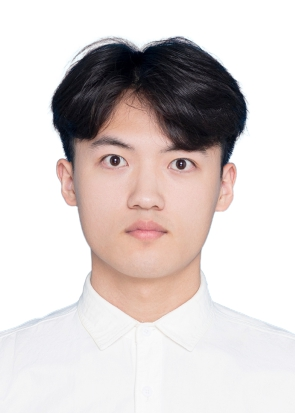
\includegraphics[width=\linewidth]{images/avatar.png}
\end{minipage}
\vspace{-0.60em}

\section[教育背景]{\sectionIcon{\faGraduationCap}{教育背景}}
\begin{itemize}
    \item {\textbf{控制科学与工程硕士，江南大学}}（\hl{中国科学院沈阳自动化研究所 · 机器人与智能系统全国重点实验室联合培养}） \hfill {2024.06--2027.06}
    \item {\textbf{自动化学士，郑州轻工业大学}} \hfill {2020.09--2024.06}
\end{itemize}

% 专业技能
\section[专业技能]{\sectionIcon{\faWrench}{专业技能}}
\begin{itemize}
    \item \textbf{视觉感知}：Grounding DINO、Qwen3-VL、YOLO11s-seg、Ultralytics YOLO、开放词汇检测、细粒度属性识别、目标检测、实例分割、视觉 Embedding 检索。
    \item \textbf{训练与后训练}：PyTorch、Transformer、Attention、CNN、Conformer、LLaMA-Factory（LoRA / 全参数 SFT）、GRPO、Qwen3-VL-8B、4 机 8 卡 H20 多机多卡训练。
    \item \textbf{端侧部署}：TensorRT、ONNX、NVIDIA Jetson AGX Orin、CUDA、模型量化与算子优化。
    \item \textbf{数据闭环}：规则 Tagger、回灌数据挖掘、标签验收与质检、Corner Case 挖掘与合成、标签库建设、训练/验证/测试集划分。
    \item \textbf{工程与仿真}：Python、C++、Linux / Ubuntu、Git、bash、Docker、ROS2、MuJoCo、Sim-to-Real 联调。
    \item \textbf{方向储备}：激光雷达 / 摄像头 / 毫米波雷达融合、BEV Perception、Occupancy、矿山扬尘 / 浓雾 / 雨雪 / 夜间复杂工况。
\end{itemize}

% 实习经历
\section[实习经历]{\sectionIcon{\faBriefcase}{实习经历}}
{\small\textbf{CARIZON（大众×地平线合资智驾）}}\quad 感知数据部门算法实习生 \hfill {2026.06--至今}\\
{\scriptsize\color{WHU_Blue} 道路视觉感知 / 目标检测与属性识别 / 复杂工况样本合成 / 多模态后训练}
\begin{itemize}
    \item \textbf{道路目标定位与细粒度属性识别}：面向红绿灯、交通标识、车辆、行人、锥桶等道路目标，采用 Grounding DINO 开放词汇检测 + 专用 VLM 识别细粒度属性，结合视觉 Embedding 检索召回相似样本，形成\hl{“目标检测—属性理解—相似样本召回”感知数据链路}，直接支撑感知模型训练数据与标签库建设。
    \item \textbf{Tagger 挖掘 + 复杂工况样本合成}：融合车载多路传感器与回灌数据设计规则化挖掘算子，红绿灯自车转向 Tagger 在 3W 条路口数据中筛选 3K 条 CLIP，\hl{验收 90\%、挖掘召回提升 10\%}；针对废弃地面箭头/引导线等 Corner Case 设计"规则渲染 + 生成模型"合成 pipeline \hl{生成 5K 训练样本}，方法可迁移至矿山扬尘、浓雾、雨雪等复杂工况的鲁棒性数据补齐。
    \item \textbf{多模态检测/属性模型后训练}：负责泊车障碍物识别模型优化，筛选 1.8 万张挡轮杆图像完成数据清洗、标注校验与 Prompt 迭代，基于 Qwen3-VL-8B + LLaMA-Factory \hl{在 4 机 8 卡 H20 完成全参数 SFT}，完成模型二次精标业务交付。
\end{itemize}

\vspace{0.30em}
{\small\textbf{优奇智能科技有限公司（优必选子公司）}}\quad 人形机器人感知算法实习生 \hfill {2026.02--2026.05} \\
{\scriptsize\color{WHU_Blue} R11 接待机器人 / 目标检测 \& 语义分割 / Jetson AGX Orin 端侧部署 / TensorRT 推理加速}
\begin{itemize}
    \item \textbf{Jetson AGX Orin 端侧部署与推理加速}：负责 R11 接待机器人感知模型在 NVIDIA Jetson AGX Orin 端侧计算平台的部署，围绕 TensorRT 推理引擎完成 PyTorch $\rightarrow$ ONNX $\rightarrow$ TensorRT 模型转换、量化与算子性能优化，\hl{推理延迟降低 20\%}，在真机跑通检测/分割实时推理链路，形成\hl{“训练—部署—实机验证”端到端工程闭环}，积累端侧算子适配、性能调优与工程落地经验。
    \item \textbf{检测/分割模型训练与数据闭环}：基于 Python / PyTorch / Ultralytics YOLO 完成 R11 接待机器人 YOLO11s-seg 目标检测 + 实例分割训练配置、参数调整、Ubuntu 环境实验链路搭建；负责多场景数据清洗、类别一致性质检与训练/验证/测试划分，围绕误检漏检与分割边界 bad case 归因，驱动\hl{“评估—归因—数据改进”感知模型迭代闭环}。
\end{itemize}

\vspace{0.04em}
\section[科研与项目经历]{\sectionIcon{\faFlask}{科研与项目经历}}
{\small\textbf{面向具身智能灵巧操作的肌电-力融合感知与灵巧手抓取控制系统（灵心巧手） · 负责人}} \hfill {2025.02--2026.02} \\
{\scriptsize\color{WHU_Blue} 多传感器融合 / MuJoCo 仿真 / Sim-to-Real / ROS2}

\vspace{0.15em}
面向 Linker Hand G20 灵巧手搭建视觉 + 多通道物理信号（sEMG、力/触觉）+ MuJoCo 仿真多传感器融合实验系统：完成多通道高频同步采集、时间戳对齐与任务标注；基于 PyTorch 开展 Transformer / 轻量 Conformer 时序特征建模，设计视觉—仿真策略—力前馈—触觉闭环分层感知与控制链路，通过 ROS2 模块化接口打通仿真—真机联调，构成 \hl{Sim-to-Real 端到端方案雏形}，方法可迁移至激光雷达 + 摄像头 + 毫米波雷达多传感器感知融合与真机部署闭环。

\vspace{0.10em}
在机器人与智能系统全国重点实验室（中国科学院沈阳自动化研究所）承担课题实验链路组织与训练环境保障：负责传感器准备、通道配置、训练配置管理与结果检查，独立完成 \hl{Linux 训练服务器搭建与维护}；梳理多传感器融合与人机交互文献（含 BEV Perception / Occupancy 方向），\hl{支撑 IEEE Sensors Journal 综述写作}与技术路线判断。

\section[论文与研究成果]{\sectionIcon{\faBook}{论文与研究成果}}
三篇工作构成\hl{「综述定路线 — 算法破难点 — 系统做闭环」}的完整研究链条：
\begin{itemize}
    \item \hl{已中（JCR 一区 / 中科院二区）} Liang B., et al. \textit{Sensing Technologies for Hand Gesture Recognition in Human-Robot Interaction: A Review}. IEEE Sensors Journal, 2025, 26(2): 1501-1519. \textbf{综述}：梳理数据手套、视觉与肌电等手势感知路线，对比精度、侵入性与成本取舍。
    \item \hl{在修（JCR 一区 / 中科院二区 Top）} \textit{sEMG Conformer: Synergizing Local-Global Spatiotemporal Features for Continuous Force Estimation}. Biomedical Signal Processing and Control. \textbf{算法核心}：卷积局部感受野 + 自注意力全局建模，解码肌电—指尖力映射，单模型支持力等级分类与连续力值回归。
    \item \hl{在投（JCR 一区 / 中科院二区）} \textit{Dexterous Hand Grasping Control Based on Multimodal Sensory Fusion and Simulation Reinforcement Learning}. \textbf{系统闭环}：MuJoCo 仿真强化生成抓取姿态，融合视觉、肌电与触觉构建分层控制链路，G20 上完成闭环部署验证。
\end{itemize}

% 荣誉与综合素质
\section[荣誉与综合素质]{\sectionIcon{\faStar}{荣誉与综合素质}}
\begin{itemize}
    \item \textbf{中国机器人大赛暨 RoboCup 机器人世界杯中国赛} \hl{国家三等奖}；校一等奖学金（2025.10、2026）；优秀毕业生（2024.06）；优秀班干部（2022.10）。
    \item 曾任本科班长、硕士党支部书记，具备需求收集、任务拆解、协同沟通和事项推进经验。
\end{itemize}

\end{document}
